% --------------------------------------------------------------
% This is all preamble stuff that you don't have to worry about.
% Head down to where it says "Start here"
% --------------------------------------------------------------

\documentclass[10pt]{article}

\usepackage[margin=2cm]{geometry}
\usepackage{amsmath,amsthm,amssymb}
\usepackage{setspace}
\usepackage{parselines}
\newcommand{\N}{\mathbb{N}}
\newcommand{\Z}{\mathbb{Z}}
\newcommand{\R}{\mathbb{R}}
\newcommand{\al}{\alpha}
\newcommand{\h}{\hfill}

\usepackage{mathtools}
\DeclarePairedDelimiter{\ceil}{\lceil}{\rceil}
\DeclarePairedDelimiter{\floor}{\lfloor}{\rfloor}

\newenvironment{theorem}[2][Theorem]{\begin{trivlist}
\item[\hskip \labelsep {\bfseries #1}\hskip \labelsep {\bfseries #2.}]}{\end{trivlist}}

\newenvironment{prove}[2][Prove]{\begin{trivlist}
\item[\hskip \labelsep {\bfseries #1}\hskip \labelsep {\bfseries #2.}]}{\end{trivlist}}

\newenvironment{conjecture}[2][Conjecture]{\begin{trivlist}
\item[\hskip \labelsep {\bfseries #1}\hskip \labelsep {\bfseries #2.}]}{\end{trivlist}}

\newenvironment{answer}[2][Answer]{\begin{trivlist}
\item[\hskip \labelsep {\bfseries #1}\hskip \labelsep {\bfseries #2.}]}{\end{trivlist}}

\newenvironment{lemma}[2][Lemma]{\begin{trivlist}
\item[\hskip \labelsep {\bfseries #1}\hskip \labelsep {\bfseries #2.}]}{\end{trivlist}}

\newenvironment{exercise}[2][Exercise]{\begin{trivlist}
\item[\hskip \labelsep {\bfseries #1}\hskip \labelsep {\bfseries #2.}]}{\end{trivlist}}

\newenvironment{problem}[2][Problem]{\begin{trivlist}
\item[\hskip \labelsep {\bfseries #1}\hskip \labelsep {\bfseries #2.}]}{\end{trivlist}}

\newenvironment{question}[2][Question]{\begin{trivlist}
\item[\hskip \labelsep {\bfseries #1}\hskip \labelsep {\bfseries #2.}]}{\end{trivlist}}

\newenvironment{corollary}[2][Corollary]{\begin{trivlist}
\item[\hskip \labelsep {\bfseries #1}\hskip \labelsep {\bfseries #2.}]}{\end{trivlist}}

\makeatletter
\renewenvironment{proof}[1][\proofname]{\par
\pushQED{\qed}
\normalfont \topsep6\p@\@plus6\p@\relax
\trivlist
\item[\hskip\labelsep\itshape#1\@addpunct{.}]\mbox{}\\*}{\popQED\endtrivlist\@endpefalse}
\makeatother

\makeatletter
\renewenvironment{answer}[1][Answer]{\par
\normalfont \topsep6\p@\@plus6\p@\relax
\trivlist
\item[\hskip\labelsep\itshape#1\@addpunct{.}]\mbox{}\\*}{\popQED\endtrivlist\@endpefalse}
\makeatother

\makeatletter
\renewenvironment{conjecture}[1][Conjecture]{\par
\normalfont \topsep6\p@\@plus6\p@\relax
\trivlist
\item[\hskip\labelsep\itshape#1\@addpunct{.}]\mbox{}\\*}{\popQED\endtrivlist\@endpefalse}
\makeatother

\doublespacing
\begin{document}

\title{Proof Portfolio}%replace X with the appropriate number
\author{Justin Yedinak\\ %replace with your name
	MATH 245} %if necessary, replace with your course title

\maketitle

% --------------------------------------------------------------
%                         Start here
% --------------------------------------------------------------

\begin{question}{1}
	An integer $a$ is said to be a type 0 integer if there exists an integer $n$ such that $a = 3n$. An integer $a$ is said to be a type 1 integer if there exists an integer $n$ such that $a = 3n + 1$. An integer $a$ is said to be a type 2 integer if there exists an integer $n$ such that $a = 3n + 2$. \\ Prove that if $a$ and $b$ are both type 2 integers, then $ab$ is a type 1 integer.
	\begin{proof}
		Let $a$ and $b$ both be type 2 integers; that is, $a = 3m + 2$ and $b = 3 n + 2$ for some $m,n \in \Z$. We wish to show $ab$ is a type 1 integer, directly. Using substitution and algebra,
		\begin{align*}
			ab & =  (3 m + 2)(3 n + 2)        \\
			   & =  9mn + 6m + 6n +  4        \\
			   & =  9mn + 6m + 6n +  3 + 1    \\
			   & =  3(3mn + 2m + 2n +  1) + 1
		\end{align*}
		By the closure property of addition $3mn + 2m + 2n +  1$ is an integer, thus $ab$ is of type 1, as desired.
	\end{proof}
\end{question}

\newpage
\begin{question}{2}
	Use induction to prove the Wallis Sine Formulas:
	\begin{align*}
		 & \int_0^{\pi / 2} \sin^{2n} x dx = \frac{1 \cdot 3 \cdot 5 \cdots (2n-1)}{2 \cdot 4 \cdot 6 \cdots (2n)} \frac{\pi}{2}   \\
		\text{and}                                                                                                                 \\
		 & \int_0^{\pi / 2} \sin^{2n+1} x dx = \frac{1 \cdot 3 \cdot 5 \cdots (2n)}{2 \cdot 4 \cdot 6 \cdots (2n+1)} 
	\end{align*}

	\begin{proof}
		Let $x \in \R$ and $m, n \in \N$.
		In calculus, it can be shown that
		\begin{align*}
			(1) \qquad \int \sin^2 x dx = \frac x 2 - \frac 1 2 \sin x \cos x + C.
		\end{align*}
		Assume the following formula can be obtained by integration by parts
		\begin{align*}
			(2) \qquad \int \sin^m x dx = - \frac 1 m \sin^{m-1} x \cos x + \frac{m - 1}{m} \int \sin^{m-2} xdx.
		\end{align*}
		We will use induction to prove the Wallis Sine Formulas:
		\begin{align*}
			 & (3) \qquad \int_0^{\pi / 2} \sin^{2n} x dx = \frac{1 \cdot 3 \cdot 5 \cdots (2n-1)}{2 \cdot 4 \cdot 6 \cdots (2n)} \frac{\pi}{2}   \\
			\text{and}                                                                                                                            \\
			 & (4) \qquad \int_0^{\pi / 2} \sin^{2n+1} x dx = \frac{1 \cdot 3 \cdot 5 \cdots (2n)}{2 \cdot 4 \cdot 6 \cdots (2n+1)} 
		\end{align*}
		\noindent
		We will prove both equations (3) and (4) inductively by separate cases. \\ Case 1 will demonstrate equation (3) by using equation (2) where $m$ is even; that is, $m = 2n$ for each $n \in \N$. \\ Case 2 will demonstrate equation (4) by using equation (2) where $m$ is odd; that is, $m = 2n + 1$ for each $n \in \N$.

		\newpage \noindent
		% CASE1 ---------------------------------------------------------------------------------------------
		$\textbf{Case }1.$ \\
		We will prove equation (3) by induction. \\
		First we will find our anchor case, $S_1$, where $n = 1$. Notice this is the same as formula $(1)$. So,
		\begin{align*}
			(S_1) \qquad \int^{\pi / 2}_{0} \sin^2 xdx & = \frac x 2 - \frac 1 2 \sin x \cos x \Big|^{\pi / 2}_{0}                                                                                                      \\
			                                           & = \Big[\frac \pi  2 \cdot \frac 1 2 - \frac 1 2 \sin \Big(\frac \pi 2\Big) \cos \Big(\frac \pi 2\Big)\Big] - \Big[\frac 0 2 - \frac 1 2 \sin (0) \cos (0)\Big] \\
			                                           & = \Big[\frac \pi  4 - \frac 1 2 (1) (0)\Big] - \Big[- \frac 1 2 (0)(1)\Big]                                                                                    \\
			                                           & = \Big[\frac \pi  4 - 0 \Big] + 0                                                                                                                              \\
			                                           & = \frac \pi  4.
		\end{align*}
		Assume (3) holds for $S_n$. Now we wish to show that $S_{n+1}$ is true; that is, we wish to show that
		\begin{align*}
			(S_{n + 1}) \qquad \int^{\pi / 2}_0 \sin^{2(n+1)} x dx & = - \frac 1 {2(n+1)} \sin^{{2(n+1)}-1} x \cos x \Big|^{\pi / 2}_{0}+ \frac{{2(n+1)} - 1}{{2(n+1)}} \int^{\pi / 2}_0 \sin^{{2(n+1)}-2} xdx \\
			                                                       & = - \frac 1 {2n+2} \sin^{{2n+2}-1} x \cos x \Big|^{\pi / 2}_{0}+ \frac{{2n+2} - 1}{{2n+2}} \int^{\pi / 2}_0 \sin^{{2n+2}-2} xdx           \\
			                                                       & = - \frac 1 {2n+2} \sin^{2n+1} x \cos x\Big|^{\pi / 2}_{0} + \frac{2n+1}{2n+2} \int^{\pi / 2}_0 \sin^{2n} xdx                             \\
			                                                       & = \frac{2n+1}{2n+2} \int^{\pi / 2}_0 \sin^{2n} xdx
		\end{align*}
		\noindent
		Notice the induction hypothesis $S_n= \int^{\pi / 2}_0 \sin^{2n} xdx$. So,
		\begin{align*}
			 & =  \frac{2n+1}{2n+2} \Big(\frac{1 \cdot 3 \cdot 5 \cdots (2n-1)}{2 \cdot 4 \cdot 6 \cdots (2n)}\Big) \frac{\pi}{2}         \\
			 & =  \frac{2n+2 - 1}{2(n+1)} \Big(\frac{1 \cdot 3 \cdot 5 \cdots (2n-1)}{2 \cdot 4 \cdot 6 \cdots (2n)}\Big) \frac{\pi}{2}   \\
			 & =  \frac{2(n+1) - 1}{2(n+1)} \Big(\frac{1 \cdot 3 \cdot 5 \cdots (2n-1)}{2 \cdot 4 \cdot 6 \cdots (2n)}\Big) \frac{\pi}{2} \\
			 & =  \frac{1 \cdot 3 \cdot 5 \cdots (2n-1)(2(n+1) - 1)}{2 \cdot 4 \cdot 6 \cdots (2n)(2(n+1))} \frac{\pi}{2}
		\end{align*}
		as desired. Now we will prove case 2.

		% CASE2 ---------------------------------------------------------------------------------------------
		\newpage
		\noindent
		$\textbf{Case }2.$ \\
		We will prove equation (4) by induction. \\
		First we will find our anchor case, $S_1$, where $n = 1$. Notice this is the same as formula $(1)$. So,
		\begin{align*}
			(S_1) \qquad \int^{\pi / 2}_{0} \sin^{3} xdx & = \frac{2}{2+1} \int^{\pi / 2}_0 \sin^{2-1} xdx \\
			                                             & = \frac{2}{3} \int^{\pi / 2}_0 \sin^{1} xdx     \\
			                                             & = \frac{2}{3}
		\end{align*}
		Assume (4) holds for $S_n$. Now we wish to show that $S_{n+1}$ is true; that is, we wish to show that
		\begin{align*}
			(S_{n + 1}) \qquad \int^{\pi / 2}_0 \sin^{2(n+1)+1} x dx & = - \frac 1 {2(n+1)+1} \sin^{{2(n+1)+1}-1} x \cos x \Big|^{\pi / 2}_{0} + \frac{{2(n+1)+1} - 1}{{2(n+1)+1}} \int^{\pi / 2}_0 \sin^{{2(n+1)+1}-2} xdx \\
			                                                         & = - \frac 1 {2n+2+1} \sin^{2n+2} x \cos x \Big|^{\pi / 2}_{0} + \frac{2n+2+1-1}{2n+2+1} \int^{\pi / 2}_0 \sin^{2n+2+1-2} xdx                         \\
			                                                         & = - \frac 1 {2n+3} \sin^{2n+2} x \cos x \Big|^{\pi / 2}_{0} + \frac{2n+2}{2n+3} \int^{\pi / 2}_0 \sin^{2n+1} xdx                                     \\
			                                                         & = - \frac 1 {2n+3} \sin^{2n+2} x \cos x \Big|^{\pi / 2}_{0} + \frac{2n+2}{2n+3}   \int^{\pi / 2}_0 \sin^{2n+1} xdx                                                      \\
                                                                     & =  \int^{\pi / 2}_0 \sin^{2n+1} xdx \cdot \frac{2n+2}{2n+3} 
        \end{align*}
        Notice the induction hypothesis $S_n= \int^{\pi / 2}_0 \sin^{2n + 1} xdx$. So,
		\begin{align*}
			 & =  \frac{1 \cdot 3 \cdot 5 \cdots (2n)}{2 \cdot 4 \cdot 6 \cdots (2n+1)}\cdot \frac{2n+2}{2n+3} \\
			 & =  \frac{1 \cdot 3 \cdot 5 \cdots (2n)(2n+2)}{2 \cdot 4 \cdot 6 \cdots (2n+1)(2n+3)} \\
			 & =  \frac{1 \cdot 3 \cdot 5 \cdots (2n)(2(n+1))}{2 \cdot 4 \cdot 6 \cdots (2n+1)(2(n+1)+1)}
		\end{align*}
		as desired. Thus we have shown both cases, proving the Wallis Sine Formulas; that is, equations (3) and (4).
	\end{proof}
\end{question}

\newpage

\begin{question}{3}
	If a (right, circular) cylinder is circumscribed about a sphere of radius $r$ so that the cylinder has radius $r$ and height $h = 2r$ as shown below,

	\begin{figure}[h!]
		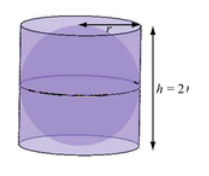
\includegraphics[width=.21\linewidth]{assets/cylinder.png}
		\centering
	\end{figure}
	\noindent
	then the total surface area of this cylinder is equal to $x$ times the surface area of the sphere and the volume of this cylinder is $y$ times the volume of the sphere.

	You will need to know the following formulae:
	\begin{align*}
		% \text{Circumference of a Circle} & = 2 \pi r \qquad     & \text{Area of a Circle}          & = \pi r^2              \\
		\text{Area (Surface) of Cylinder} & =  2 \pi r^2 + 2\pi rh \qquad & \text{Area (Surface) of Sphere} & =  4 \pi r^2         \\
		\text{Volume of Cylinder}         & =  \pi r^2 h                  & \qquad \text{Volume of Sphere}  & =  \frac 4 3 \pi r^3
	\end{align*}

	\begin{proof}
		Suppose a (right, circular) cylinder is circumscribed about a sphere of radius $r$ so that the cylinder has radius $r$ and height $h = 2r$. We wish to show the total surface area of this cylinder, $S_C$, is equal to some real number $x$ times the surface area of the sphere, $A_S$, and the volume of this cylinder, $V_C$, is $y$ times the volume of the sphere, $V_S$, where $x,y \in \R$. Now, let that $x = 3/2$ and $y = 3/2$; that is, we want to show
		\begin{align*}
			A_C = \frac{3}{2} \cdot A_S \quad \text{and} \quad V_C = \frac{3}{2} \cdot V_S
		\end{align*} We will now prove the above statements. First, we will show that $A_C = \frac 3 2 \cdot A_S$. Recall $h = 2r$ and so by the respective formulae we have,
		\begin{align*}
			\frac 3 2 \cdot 4 \pi r^{2} & = \frac {12}{2} \pi r^{2}    \\
			                            & = 6 \pi r^{2}                \\
			                            & = 2 \pi r^{2}  + 4 \pi r^{2} \\
			                            & = 2 \pi r^{2}  + 2 \pi r(2r) \\
			                            & = 2 \pi r^{2}  + 2 \pi rh
		\end{align*}
		as desired. Now, we will show that $V_C = \frac 3 2 \cdot V_S$. Recall $h = 2r$ and so by the respective formulae we have,
		\begin{align*}
			\frac 3 2 \cdot \frac 4 3 \pi r^3 & = \frac{12}{6} \pi r^3 \\
			                                  & = 2 \pi r^3            \\
			                                  & = \pi r^2 (2r)         \\
			                                  & = \pi r^2 h
		\end{align*}
		as desired. We have shown that the total surface area of this cylinder is equal to some $\frac 3 2$ times the surface area of the sphere and the volume of this cylinder is $\frac 3 2$ times the volume of the sphere.
	\end{proof}
\end{question}

\vspace{5mm}

\begin{question}{4}
	For all integers $a$ and $b$, $a \equiv b \mod 5$ if and only if $(a + 3b) \equiv (3a + b) \mod 10$.
	\begin{proof}
		Let $a, b \in \Z$. We seek to demonstrate that $a \equiv_{5} b$ if and only if $(a + 3b) \equiv_{10} (3a + b)$. \\ Now we will show the forward implication; that is, if $a \equiv_{5} b$, then $(a + 3b) \equiv_{10} (3a + b)$.
		This is equivalent to if $5 \mid (a -b)$, then $10 \mid ((a+3b)- (3a +b))$.
		It follows that there exists an integer $c$ such that $5c = a - b$. So,
		\begin{align*}
			(a +3b) - (3a + b) & = a +3b - 3a - b      \\
			   & = a - b + 3b - 3a     \\
			   & = a - b + -3(a -b  )
		\end{align*}
		Now we substitute $5c$ for $a - b$, yielding $5c + -3(5c  ) = 10(-c)$. Of course $10$ is evenly divides $10(-c)$, thus showing the forward implication.
		Next, we will show the backward implication; that is, if $10 \mid ((a + 3b) - (3a + b))$, then $5 \mid (a -b)$.
		It follows that there exists an integer $d$ such that
		\begin{align*}
			10d & = (a + 3b) - (3a + b) \\
			    & = a + 3b  -3a - b     \\
			    & = a -3a + 3b   - b    \\
			    & = a(1 - 3) - b(1-3)   \\
			    & =  (1 - 3)(a- b)      \\
			    & =  (- 2)(a- b)
		\end{align*}
		Now we divide by $-2$, yielding $-5d= a- b$. Since $5 \mid -5d$, then clearly $5 \mid (a -b)$.
		Thus, we have shown that $a \equiv b \mod 5$ if and only if $(a + 3b) \equiv (3a + b) \mod 10$.
	\end{proof}
\end{question}

\newpage

\begin{question}{5}
	Let $\sim$ be a relation on $Z$ given by $a \sim b$ if and only if $2$ divides $a+b$. Prove that $\sim$ is an equivalence relation.
	\begin{proof}
		Let $a, b \in \Z$. Suppose $\sim$ is a relation on the integers such that $a \sim b$ if and only if $2 \mid (a + b)$. We wish to show that $\sim$ is an equivalence relation; that is, we want to show $\sim$ is reflexive, transitive, and symmetric.
		For any given $a \in \Z$, we have $a \sim a$ since $a+a =2a$ and $2 \mid 2a$; and thus $\sim$ is reflexive.
        Next we will show $\sim$ is transitive. For each integer $a$, $b$, and $c$, $a \sim b$ and $b \sim c$, then $2 \mid (a + b)$ and $2 \mid (b + c)$. Thus, it follows that there exists integers $m$ and $n$ such that $2m = a + b$ and $2n=b +c$. Since $a + c = (2m -b) + (2n -b) = 2(m-b)$. By closure of integer addition $m-b$ is an integer, thus $2 \mid (a +c)$ and $\sim$ is transitive. Now we will show $\sim$ is symmetric. For any given integers $a$ and $b$, if $a \sim b$, then $b \sim a$. This is true since $a + b = b + a$ by the commutative property of addition. Thus, we have shown $\sim$ is an equivalence relation.
	\end{proof}
\end{question}

\vspace{1mm}


\begin{question}{6}
	Let $a, b \in Z$, not both equal to $0$, and let $d = gcd(a, b)$.\\
	(a) $\quad$ Use the Fundamental Theorem of Arithmetic to explain why $\frac a d$ and $\frac b d$ are integers. \\
	(b) $\quad$ Prove that $gcd(\frac a d, \frac b d) = 1$.
    \begin{proof}
		We will first prove $(a)$. Let $a, b \in Z$, not both equal to $0$, and let $d = gcd(a, b)$. We wish to show that $\frac a d$ and $\frac b d$ are integers. Let's rewrite $a$ and $b$ as factorizations of distinct prime numbers, $p$. So, $a = p_1^{a_1} \cdot p_2^{a_2} \cdots p_k^{a_k}$ and $b = p_1^{b_1} \cdot p_2^{b_2} \cdots p_k^{b_k}$ where each $a_k$ and each $b_k$ $(k \in \N)$ is a whole number. Then by corollary 3.3.4, $d = gcd(a,b) = p_1^{\text{min}\{a_1,b_1\}} \cdot p_2^{\text{min}\{a_2,b_2\}} \cdots p_k^{\text{min}\{a_k,b_k\}}$. Now let's divide by the prime factorizations of $a$ by $d$; that is, 
		\begin{align*}
			\frac {a}{gcd(a,b)} &= \frac {p_1^{a_1} \cdot p_2^{a_2} \cdots p_k^{a_k}}{p_1^{\text{min}\{a_1,b_1\}} \cdot p_2^{\text{min}\{a_2,b_2\}} \cdots p_k^{\text{min}\{a_k,b_k\}}}\\
			&= p_{1}^{[a_1 - \text{min}\{a_1,b_1\}]} \cdot p_{2}^{[a_2 - \text{min}\{a_2,b_2\}]} \cdots p_{k}^{[a_k - \text{min}\{a_k,b_k\}]}
		\end{align*}
		Notice that since both $a_k$ and $b_k$ are integers, the minimum value will also be an integer; furthermore, it will be an integer less than or equal to both $a_k$ and $b_k$. Thus, it follows that the difference for each $a_k$ and $\text{min}\{a_k,b_k\}$ will be a nonnegative integer. Therefore we have a prime factorization of $\frac a d$. Since multiplication is closed under the integers or primes, $\frac a d$ is an integer. We can argue similarly that $\frac b d$ is an integer.
		\vspace{5mm} \\ 
        Now we will prove $(b)$, that $gcd(\frac a d , \frac b d) = 1$. We seek to show that $gcd(\frac a d , \frac b d) = r$, eventually showing $r =1$. Suppose to the contrary that $r \neq 1$ and instead $r \in \N \setminus \{1\}$. From the definition of the greatest common divisor we know that if $gcd(\frac a d , \frac b d) = r$, then $\frac a d = mr$ and $\frac b d = nr$ where $m,n \in \Z$. So, $a = mdr$ and $b = ndr$, thus $dr$ is a common divisor of both $a$ and $b$. This is a contradiction by our initial assumption that $gcd(a,b)=d$ since $dr > d$ and the definition of the greatest common divisor prescribes that $dr \le d$. It follows that $r = 1$.
    \end{proof}

\end{question}

\newpage

\begin{question}{7}
Persistence: Pick one proof that you have worked on this semester that you struggled to understand and solve, and explain how the struggle itself was valuable. In the context of this question, describe the struggle and how you overcame the struggle. You might also discuss whether struggling built aspects of character in you (e.g. endurance, self-confidence, competence to solve new problems) and how these virtues might benefit you in later ventures, mathematical or otherwise. Now that you have more knowledge, rewrite the proof. Include a copy of your original attempt. (You do not need to rewrite or “neaten” up your original attempt.)\\

Mathematical induction in general and especially this next problem (from homework 5 question 9) has given me trouble. Prove Bernoulli's inequality: If $ \al > -1, \al \neq 0$, then $(1 + \al )^n > 1 + n \al$ for all natural numbers $n> 1$. Here is my original attempt:
    \begin{proof}
        Let $\al > -1$ and $\al \neq 0$. Suppose the statement $S_n: (1 + \al )^n > 1 + n \al$ for all $n \in \N \setminus \{1\}$. We will use mathematical induction. Note the anchor case holds; that is, $S_2: (1+ \al)^2 = \al^2 +2\al + 1> 1 + 2 \al$ subtracting the right side gives $\al^2 > 0$. Now let's suppose $S_{n+2}$ is true; that is we wish to show that
        \begin{align*}
            (1 + \al )^{(n+2)}                  & > 1 + \al (n+2)                           \\
            (1 + \al )^{n} \cdot (1 + \al )^{2} & > 1 + \al n+ 2 \al                        \\
            (1 + \al )^{n}                      & > \frac{1 + \al n+ 2 \al}{(1 + \al )^{2}}
        \end{align*}
        But from $S_n$
        \begin{align*}
            (1 + \al )^{n}  > 1+ \al n & \ge \frac{1 + \al n+ 2 \al}{(1 + \al )^{2}}
        \end{align*}
	\end{proof} \noindent
Through studying several examples of induction proofs and appreciating comments on my previous work, I have improved my understanding of mathematical induction and this proof. This is my improved version: 
\begin{proof}
	Let $\al > -1$ and $\al \neq 0$. Suppose the statement $S_n: (1 + \al )^n > 1 + n \al$ for all $n \in \N \setminus \{1\}$. We will use mathematical induction. Note the anchor case holds; that is, $S_2: (1+ \al)^2 = \al^2 +2\al + 1> 1 + 2 \al$ since $\al^2 > 0$. By assumption $\al \neq 0$, restricting the inequality. Assume this holds for $S_n$. Now we wish to show that $S_{n+1}$ is true; that is, we wish to show that
	\begin{align*}
		(1 + \al )^{n+1} &> 1 + \al(n + 1)
	\end{align*}
	Since $\al > -1$ this implies $(1+\al)$ will be nonnegative, maintaining the inequality in the following operation. Multiply $(1+\al)$ to both sides of the induction hypothesis inequality yields
	\begin{align*}
		(1+\al)(1 + \al )^n &> (1 + n \al)(1+\al) \\
		(1 + \al )^{n+1} &> 1+n\al+\al+n\al^2 \\
		(1 + \al )^{n+1} &> 1+\al(n+1)+n\al^2
	\end{align*}
	We know $na^2$ is a nonnegative number since $a^2$ and $n \in \N \setminus \{1\}$ must both be nonnegative. So we can drop $na^2$, still maintaining the inequality. Thus
	\begin{align*}
		(1 + \al )^{n+1} &> 1+\al(n+1).
	\end{align*}

\noindent
This shows that $S_{n+1}$ is true whenever $S_n$ is true. By the principle of mathematical induction, it follows that $S_n$ is true for every natural number $n$ besides $1$.
\end{proof}

Enduring when we don't understand something or succeed at first is an important trait, no matter the pursuit. More often than not people tend to fail at their first attempt at something. This makes persistence one of the most important traits to nurture for anyone who wants to push past their current limits. Courses that introduce new concepts or a new way of thinking is a good way to nurture persistence and prove to one's self that we can succeed.
\end{question}

\newpage

\begin{question}{8}
Creativity: Give one example of a mathematical proof from this class that you found creative, and explain what you find creative about it. For example, you can choose an instance of creativity you experienced in your own problem-solving, or something you witnessed in class or reading the book. Rewrite the statement and proof as part of your response.
\begin{answer}
I find the solutions to nonconstructive existence proofs to require some extra creativity in general. This is because we have to prove its existence without showing an example of the object. This sort of idea is analogical to mathematics in general. In my opinion mathematics is primarily beautiful because it has allowed humans to prove or determine things that we can not necessarily see. Here is an example from the textbook on page 56 theorem 2.1.13; that is, there exists a power of $7$ that has exactly $100$ digits.

\begin{proof} 
	Consider the sequence $(1,1,2,3,4,5,6,6,\dots)$ of the number of 
	digits in the powers $(1,7,49,343,2401,16807,117649,823543,\dots)$ of $7$. Observe that
	\begin{align*}
		7^{200} = (7^2)^{100} = 49^{100} > 10^{100}
	\end{align*}
	Because $10^{100}$ has $101$ digits and $7^{200}$ is even larger, $7^{200}$ must have more than $100$ digits. In particular, the $201$st term of the sequence is greater than $100$. Thus, the sequence $(1,1,2,3,4,5,6,6,\dots)$ starts below $100$ and eventually exceeds $100$. \\ \indent Next we will show that the sequence $(1,1,2,3,4,5,6,6,\dots)$ can never skip over any natural number. Specifically, if $n$ is a term in the sequence $(1,1,2,3,4,5,6,6,\dots)$, then the next term cannot be greater than or equal to $n+2$, skipping $n+1$. Indeed, if $7^k$ has $n$ digits, then $10\cdot 7^k$ has $n+1$ digits, and since
	\begin{align*}
		7^k < 7^{k+1} = 7(7^k) < 10(7^k),
	\end{align*}
	it follows that $7^{k+1}$ has either $n$ or $n+1$ digits. Thus, each subsequent term of the sequence $(1,1,2,3,4,5,6,6,\dots)$ either remains constant or increases by $1$. \\
	\indent Because $(1,1,2,3,4,5,6,6,\dots)$  starts below $100$ and increases to a number over $100$, never skipping over any natural number, the sequence must include $100$. It follows that there exist a power of $7$ with exactly $100$ digits.
\end{proof}
\end{answer}
\end{question}

\newpage

\begin{question}{9}
Disposition toward beauty: Consider one mathematical idea from the course that you have found beautiful, and explain why it is beautiful to you. Your answer should: (1) explain the idea in a way that could be understood by a classmate who has taken calculus but has not yet taken this class and (2) address how this beauty is similar to or different from other kinds of beauty that human beings encounter.
\begin{answer}
	The pigeon hole principle is beautiful because of its simplicity. Like its name suggests, its beauty is similar to the beauty that one can find in nature. It is not always visually appealing, but there is beauty in the simplicity of nature. And as such, this concept relies on the nature of nature; that is, space and matter. Probably the easiest way to understand this concept is by visualizing these spaces and material objects. \\ \indent 
	If $n + 1$ or more objects (or pigeons) of any kind are placed into an $n$ number of spaces (or holes), then there is at least one space containing two or more objects (or pigeons). \\ \space \\ 
	Here is a simple example from page 75 to aid in understanding the use case of the pigeon hole principle. Exercise 4: Show that any three integers contain a pair whose sum is even.
	    \begin{proof}
	        By the pigeon hole principle at least two of the three integers will be of the same parity (even or odd), thus there are two cases we care about. \\ \indent First, if at least two integers are even, then since both have common factors of $2$ the sum will be even. \\ \indent Secondly, if at least two integers $m$ and $n$ are odd; that is, represented as $m = 2j + 1$ and $n = 2k + 1$ where both variables $j$ and $k$ are integers. \\ Observe $m + n = 2j + 1 + 2k + 1= 2j + 2k +2 = 2(j+k+1)$. Since $j+k+1$ is an integer the sum is even.
		\end{proof}
\end{answer}
\end{question}

\vspace{5mm}

\begin{question}{10}
Imagination: How has your mathematical imagination been enhanced as a result of taking this class? Additionally, give at least one example of a question about the material that you’d like to explore further, and describe why this is an interesting question to you. \\ \indent
Taking this class has increased my analytical abilities. As a computer science major, I have used material from this course to help solve problems in my computer science course work. The logic, set, and elementary number theory have especially proved useful when writing algorithms to solve problems. Even in my writing intensive course, legal reasoning, this course has helped me to make better logical arguments and understand the more formal methods of argumentation. As to a question that interests me, when I first learned about mathematical induction it reminded me of recursion. I guess, i'd like to know how or if they are related because, as I said before, I am a computer science student first and foremost.
\end{question}

% --------------------------------------------------------------
%     You don't have to mess with anything below this line.
% --------------------------------------------------------------

\end{document}